Einstein equations very famously link the matter content of our spacetime with its geometric structure; however, Einstein equations themselves don't exclude particularly exoctic phenomena, such as causality violation or superluminal travel. In other words, if we were able to reproduce any stress-energy tensor, we could induce any space topology we were to imagine.

This statement vividly clashed with our physical intuition: here it comes then that we would like to require an additional hypothesis, one that was able to select all and only ``reasonable'' forms of matter. We would like it to be general enough so that it can include all types of known fields, but strong enough to rule out unphysical contents and have useful geometrical implications.

Unfortunately such a hypothesis doesn't exist yet; or, well, it would be better to say that there exist too many, but it is not clear wether we have already found a satisfying one or not. In this chapter we are going to quickly review the intricated set of conditions proposed, focusing on the ones that will be useful for us. 

The generalization of the area theorem proposed later on in this thesis is exactly weakening the energy condition required in Hawking's area theorem; we will focus then on motivating why such a generalization was much needed, and what brought us to the choice of the class of energy condition we will be employing.

\section{Pointwise Energy Conditions}
\label{sec:pointwise-energy-conditions}

In the following we will use the ``variational'' definition of the stress tensor:
\[
   T_{\mu\nu} = \frac{2}{\sqrt{-g}} \frac{\delta S_{mat}}{\delta g^{\mu\nu}}. 
\]

Hystorically energy conditions were introduced to deduce relativity theorems within a general framework. They have provided with a major step forward, as the regime of validity of important statements such as singularity theorems could be much widened by means of their employment. 
In particular, they were all in the form of pointwise restrictions on some contraction of the stress energy tensor, a condition general enough to be satisfied by many forms of matter.

The weakest among the energy conditions typically appearing in those classical relativity theorems is the famous Null Energy Condition. That is indeed the one assumed for Penrose's Singularity theorem and Hawking's Area theorem, so that shall also be the one we analyze with most care.

\begin{definition}
    \label{def:NEC}
    The Null Energy Condition (NEC) requires that at any point of spacetime and for any null vector \(U^{\mu}\) it holds
    \[
    T_{\mu\nu}U^{\mu}U^{\nu} \ge 0.
    \]
\end{definition}

But what does that physically mean? To assign an interpretation to this condition we need to ask for some help to Einstein's equation, and turn it into the \emph{null convergence condition}:
\[
    R_{\mu\nu}U^{\mu}U^{\nu} \ge 0. 
\]
Now, recalling Riccati inequality \eqref{eq:Riccati-ineq}, we can see that NEC would imply that a non rotating null geodesic congruence locally converges, or equivalently that gravity is attractive for particles that move along null geodesics.

This condition is the weakest in the sense that is implied by all other pointwise energy conditions, as shown by proposition \(2.2\) of \cite{kontou2020energy}; it is satisfied by the most common forms of matter in the universe, such as dust, radiation and saturated by the cosmological constant, but in the same reference \cite{kontou2020energy} it is shown that a very simple scalar fields non minimally coupled to gravity can already provide a violation of NEC.

If that wasn't convinvig enough, Kontou and Sanders report also an argument (originally by Epstein, Glaser and Jaffe \cite{epstein1965nonpositivity}) to show that \emph{any} pointwise energy condition must be violated by quantum fields. To show such result Reeh-Schlieder theorem for local observables is needed:
\begin{theorem}[Reeh-Schlieder]
    \label{th:reeh-schlieder}
    Let \(\mathcal{A}(O)\) the set of all operators of a QFT localized in a fixed region \(O\) in Minkowski space, and \(\vert \Omega \rangle\) the vacuum state. Then the set of vectors \(\mathcal{A}(O)\vert \Omega \rangle\) is dense in the Hilbert space \(\mathcal{H}\).
\end{theorem}

Hence it immediately follows that (\cite{epstein1965nonpositivity})
\begin{theorem}
    \label{th:quantum-violation-pointwise-conditions}
    Let \(A\in \mathcal{A}(O)\) a self-adjoint local operator of a QFT so that \(\langle \psi\vert A\vert\psi\rangle\ge 0\) for all \(\vert\psi\rangle\) in the domain of \(A\). If \(\langle \Omega\vert A\vert\Omega\rangle = 0\) then \(A \equiv 0\).
\end{theorem}
\begin{proof}
    Since \(A\ge 0\), 
    \[
        \langle \Omega\vert A\vert\Omega\rangle = \langle \Omega\vert \sqrt{A}\sqrt{A}\vert\Omega\rangle = \vert\vert \sqrt{A}\vert\Omega\rangle\vert\vert^2 = 0.
    \] 
    This implies that \(\sqrt{A}\vert\Omega\rangle = 0\) itself; but then also \(A\vert\Omega\rangle = \sqrt{A}\sqrt{A}\vert\Omega\rangle = 0\). Finally, by means of Reeh-Schlieder theorem \ref{th:reeh-schlieder} and local commutativity, we gain that \(A\) must vanish on a set of state dense in \(\mathcal{H}\), and so on all \(\mathcal{H}\).
\end{proof}

This result shouldn't come as a big surprise. It has been noticed long ago how black hole evaporation is in tension with Hawking's Area theorem, statement that asks for the null energy conditions as a hypothesis. Black hole evaporation is a quantum effect, so we should indeed expect that whenever quantum fields are included, at least one of the hypothesis of the black hole area theorem should be violated: NEC, being a statement about the stress energy tensor, is the natural candidate - even if we will see that causality itself is not immune either to the transition towards a quantum regime.

\section{Quantum Inequalities and Averaged Conditions}
Now that we know NEC won't be valid for any universe containing quantum fields, what should we replace it with? The answer to this question remained very unclear for quite a long time, until in \(1978\) Ford \cite[]{ford1978quantum} realized that in order to prevent such negative energy fluxes from violating the second law of thermodynamics, the magnitude and duration of the effect must be constrained by an inequality of the form
\begin{equation}
    \label{eq:constraint-flux}
    \vert F \vert \lesssim t_0^{-2},    
\end{equation}
where \(F\) is the flux, and \(t_0\) the time it lasts. This way, the magnitude of energy absorbed cannot exceed \(t_0\vert F\vert \lesssim t_0^{-1}\), and by the time-energy uncertainty relation no macroscopic violation occurs. Equation \eqref{eq:constraint-flux} was the first \emph{quantum energy inequality}. 

Denote as \(\rho\) the energy density, or any similar quantity that it is necessary to bound; then the most general form of a quantum energy inequality is 
\[
\langle \rho(f) \rangle_{\omega} \ge - \langle \mathcal{Q}(f) \rangle_{\omega}   
\]
where \(f\) is a suitable test function and \(\omega\) is some quantum state belonging to a class of reference states (most commonly Hadamard states for free fields).

Whenever the operator \(\mathcal{Q}(f) \) is a multiple of the identity 
\[
    \mathcal{Q}(f) = Q(f)    
\]
the QEI is said to be \emph{state independent}. Naturally this is the most amiable class of quantum energy inequalities, as the absence of a specific reference state leaves the relation the most possibly general.

Quantum energy inequalities have sometimes been described as uncertainty principle-like bounds~\cite[]{ford1998quantum}, or reminiscent of them~\cite[]{fewster1999bounds}, even if any of their proof doesn't assume or use any quantum mechanical time-energy uncertainty relation.
In their review~\cite[]{kontou2020energy} Kontou and Sanders point out that a better suiting interpretation should be instead researched within the relationship between quantum energy inequalities and the stability of the system they restrain: they should be viewed as a generalisation of having quantum mechanical system with bounded hamiltonian spectrum, \(H \ge 0\). They point out this analogy by extending to \(n = 1\) dimension the argument in~\cite[]{fewster1998bounds} (where Fewster and Eveson derive a quantum energy inequality for free scalar fields in \((n = 2)\)--Minkowski spacetime), while a more elaborate analysis can be found in~\cite[]{fewster2003stability}. Very roughly, when moving into a gravitational context, absolute energies becomes relevant - and not just differences of energies - from which arises the possibility for negative bounds, instead of having the spectrum always bounded by a \(0\). Such negative energies might be due to many subtleties, such as non trivial metrics, compactification of spatial dimensions~\cite[]{banach1979vacuum, louko1998inextendible}, or boundary conditions - such as the Casimir effect. Quantum energy inequalities however, are very difficult to formulate for interacting fields or on curved spacetime, and only a limited number of them has been proved for more than free theories, or Minkowski background. 

On the edge of the new millennium, a new conjecture came around: it has been observed by Ford and Roman in \cite[]{ford1999quantum} how local violations of pointwise energy condtions seemed to be compensated for, or even overcompensated for, in other regions of spacetime, as if some negative energy was ``borrowed'', and then payed back later in time with some ``interest''. From this analysis comes the name \emph{quantum interest} conjecture, and this lead to the formulation of \emph{averaged} energy condition.
\begin{definition}
    An \emph{averaged energy condition} is the requirement for a specific contraction of the stress energy tensor of a theory, averaged over a suitable region of spacetime, to be non negative.
\end{definition}
\begin{remark}
    Converesely from quantum energy inequalities, averaged energy conditions insist on on the lower bound \(0\), simplifying many problems that do arise for QEIs in defining such negative bounds in the case of interacting fields or curved spacetimes. At the same time they are way weaker than pointwise energy conditions, so in this sense they try to combine the best of both.
\end{remark}
In literature the region onto which the contraction of the stress tensor is averaged to obtain an energy condition is nearly always a \emph{causal geodesic}, and besides it is precisely the sort of condition that will be helpful for us.

\subsection{The Achronal Averaged Null Energy Condition}

The averaged energy conditions most interesting for us are the Averaged Null Energy condition and its achronal version.

\noindent
They ask respectively that the inequality
\begin{equation}
    \label{eq:ANEC}
    \int_{-\infty}^{+\infty} d\lambda T_{\mu\nu}U^{\mu}U^{\nu} d\lambda \ge 0    
\end{equation}
hold on any null geodesic, or on any achronal null geodesic, where \(\lambda\) is the affine parameter and \(U^{\mu}\) is the tangent field. They are - in some sense - the natural generaization of the Null Energy Condition, and benefit of a very wide range of validity. 
\noindent
Indeed ANEC in Minkowski can only be violated by non minimally coupled fields if they take trans-Planckian values, and even the Casimir effect doesn't invalidate it.
However, a counterexample that lies very close to our field of interest is provided by \cite[]{levi2016versatile}, where Levi and Ori numerically compute the renormalized stress tensor for minimally coupled scalar fields in a Schwarzschild background, and show that ANEC could be violated in that context. 
Even there instead AANEC keeps holding: the only known counter examples to this condition are believed unphysical, as they all involve Planck lenght distances, where the validity of QFT in curved spacetimes and semiclassical quantum gravity encounter its limit. This is suggesting that AANEC might be actually a consequence of some fundamental properties of a full theory of quantum gravity: the bridge towards such yearned for theory is the main motivation for its study, and has made of it the ultimate graal of energy conditions.

More precisely, the two forumlations of the condition given by Kontou and Sanders are:
\begin{itemize}
    \item[\ding{99}] In Minkowski space the ANEC holds for any reasonable QFT with a stress tensor which (locally) generates the translations of the theory.
    \item[\ding{99}] On-shell configurations can violate AANEC only over Planck scale distances in directions transversal to the null geodesic.
\end{itemize}
The second formulation is clearly at least slightly stronger, and is the one with the widest range of interest for approaches to semi-classical gravity. By weakening any of the hypothesis, such as the on-shell requirement or the achronality, counterexamples can be provided, from which this form of the condition was derived. 
There have been various attempts to prove AANEC, especially in its first formulation, that relies on various ideas borrowed from various range of backgrounds, from thermodynamics to AdS/CFT correspondence. The most interesting results so far have been attained in \(2\) dimensional specetimes:
\begin{itemize}
    \item[\ding{99}] In \(2-\)Minkowski ANEC has been proved by Verch in \cite[]{verch2000averaged} for general quantum fields with a mass gap, suggesting that the validity of this conditon goes beyond free fields.
    \item[\ding{99}] In \cite[]{wall2010proving} Wall derived AANEC from the generalized second law of thermodynamics; this derivation sounds rather paradoxical at the very least if one notices that ANEC is invariant under time inversion, while the second law cannot be.
\end{itemize}

Even if this sounds all very exciting, unfortunately no relativity theorem -including our area theorem- can be proved under energy conditions that average \(T_{\mu\nu}U^{\mu}U^{\nu}\) over the all extension of the geodesics. As we have seen, the existence criteria for focal points derived in proposition \ref{prop:fp-criteria} requires the integral to start from the surface \(P\) with respect to which the focal point will form. In order to derive our results then, we need that the geodesic segment onto which we control the contraction of \(T_{\mu\nu}\) is not infinite at both ends. 

\noindent
We are going to see in the next sections of this chapter how we weaken the condition in order to be both still reasonable and valid on non bi-infinite intervals, but it is worth pointing out that all the geodeisc segments onto which we will ask such conditions to hold are segments of achronal null geodesics, and hence - from what argued above - might have any chance to generalise our results to a proper full theory of quantum gravity.

\begin{wrapfigure}{r}{0.47\textwidth}
    \centering
    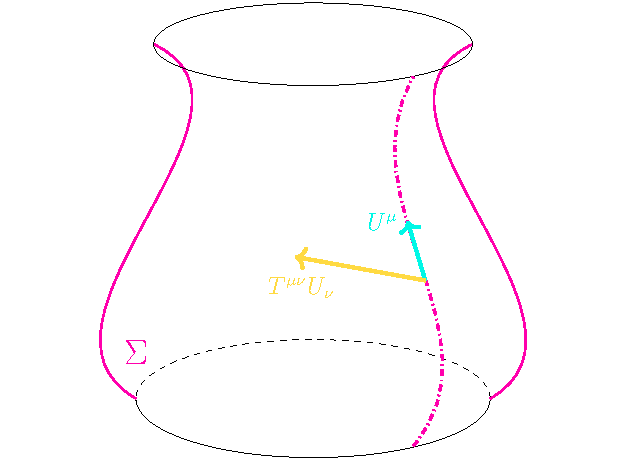
\includegraphics[scale=0.65]{Immagini/ANEC/ANEC.pdf}
    \caption{\(T_{\mu\nu}U^{\nu}\) accounts for the energy flux through the surface orthogonal to \(U^{\nu}\), which happens to be \(\Sigma\) itself because it is a null hypersurface.}
    \label{fig:ANEC}
\end{wrapfigure}

Finally, assigning a physical interpretation to energy condition is notoriously rather hard in most cases, and indeed this is the wakness that raises their loudest critics.
However, in this case Wald and Yurtsever have been able to provide a nice interpretation: in the introduction of \cite[]{wald1991general} they point out, for null hypersurfaces \(\Sigma\) generated by achronal curves \(\gamma\) with tangent field \(U^{\mu}\), remembering that for null hypersurfaces the tangent vector coincides with the normal one, \(T_{\mu\nu}U^{\mu}U^{\nu}\) is nothing but the local energy flux through \(\Sigma\).

If one assumes \eqref{eq:ANEC} to be valid for all achronal null geodesics then, it is simply requiring that the \emph{total} energy flux through any such \(\Sigma\) is non negative.

\section{Sobolev Conditions}
\label{sec:sobolev-conditions}
As mentioned in the conclusion of the above section, no relativity theorem can be proved with energy condition that average contractions of the stress tensor over \emph{full} geodesics. In particular, in order to apply the index form method we will always have to consider geodesic segments with starting point on the submanifold \(P\) we will pick.

We need to formulate an average condition that is valid on limited geodesic segments then, and if we believe AANEC to be valid, it would be unreasonable to ask for the lower bound to be zero (or positive); we are going to employ the following condition:

\begin{definition}
	We say that the \emph{Sobolev energy condition} is satisfied on a curve \(\gamma\) and for a ``time'' \(\ell\), if there exist some \(m\in \N\) and two non negative constants \(Q_0\) and \(Q_m\) such that, for any \(f\) in the Sobolev space \(W_0^m([0,\ell])\):
    \begin{equation}
        \label{eq:Sobolev-condition}
        \int_0^{\ell} f(\lambda)^2 R\langle T_{\mu\nu}\rangle_{\omega}U^{\mu}U^{\nu} d\lambda \ge -Q_m(\gamma) \vert\vert f^{(m)}\vert\vert^2 - Q_0(\gamma) \vert\vert f\vert\vert^2.
    \end{equation}
	\noindent
	We will apply this conditions to null geodesics \(\gamma\) orthogonal to some surface \(P\), where we will assume \(\lambda\) is the affine parametrization such that \(\gamma(\lambda = 0) \in P\) and \(\hat{H}_{\mu}\frac{d\gamma^{\mu}}{d\lambda}\Big\vert_{\lambda = 0} \equiv 1\) (\(\hat{H}_{\mu}\) is the versor of the mean normal curvature of \(P\)); finally, \(\vert\vert \star \vert\vert\) denotes the standard norm in \(L^2(I)\), and \(\omega\)  asuitable quantum state.
\end{definition}

The name ``Sobolev condition'' is not in use in literature, but for shortness we denoted this condition with such name as in particular makes use of Sobolev norms.
The first main reason for which we started analyzing this condition is that in section \(4\) of \cite{fewster2020new} Fewster and Kontour make use of an analogous condition to derive semi-classical singularity theorems.
Furthermore, the form of this bound is inspired to Quantum Energy Inequalities that have been proved from QFTs (refer again to the review \cite[]{kontou2020energy} for more details). In particular, because of this similarity to QEIs we will have to insist on applying it only to functions with the Dirichlet boundary conditions \(f(0) = 0 = f(\ell) \). We will see that this will cause us quite a few problems, but it is important to restrict to compactly supported functions because otherwise - apart from the mathematical convergence properties coming along - counterexample might arise easily from the presence of singular negative energy densities, as motivated in \cite[]{ford1998quantum}.

At last, even if it is true that bounds on half complete geodesics are yet to be proved, some arguments in favour of non divergence of such integrals have already been provided by many authors. To mention one that seems the most revelant for us, in \cite[]{ford1996averaged}, where Ford and Roman prove bounds of this sort for \(2\) dimensional Schwarzschild, and argue that similar results might hold in \(4\) dimensions as well.

\section{The Smeared Null Energy Condition}
\label{sec:SNEC}

In section \ref{sec:pointwise-energy-conditions} we mentioned that non minimally coupled scalar fields violate all the main pointwise energy conditions; hence, by theorem \(4.1\) of \cite[]{kontou2020energy}, the corresponding quantized field doesn't admit any of the corresponding quantum energy inequality. Nevertheless it can admit state-dependent QEIs, but this means that if we look for a condition of the form of \eqref{eq:Sobolev-condition} we will have to make a non trivial choice of \(\omega\).

Depending on the situation this might not be a big deal, nevertheless it is worth looking for state-independent results, when aiming at the highest level of generality.
In \cite[]{fewster2003null} Fewster and Roman showed that QEIs along null geodesics cannot exist in \(4\) dimensional Minkowski spacetime for the massless minimally coupled scalar field. However very recently, in \cite[]{freivogel2018smeared} Freigovel and Krommydas argued that such example is not particularly physical because it needs to pass through the creation of states from the vacuum using excitiation of arbitrary momenta. Indeed, by restricting the momenta to be below the UV cut-off of the theory, they arrive to the proposal of a new energy condition, the Smeared Null Energy condition.

\begin{definition}
	The Smeared Null Energy Condition asks that, on any achronal portion of a null geodesic it holds:
	\begin{equation}
		\label{eq:SNEC}
		\forall f \in C_0^2[(-\infty, +\infty)] \quad\quad \int f^2(\lambda)\langle T_{\mu\nu}U^{\mu}U^{\nu}(\lambda) \rangle d\lambda \ge -\frac{4B}{G_N}\vert\vert \nabla_U f\vert\vert^2
	\end{equation}
\end{definition}

Freigovel and Krommydas conjecture that this bound should always hold as long as the cut-off rule is satisfied, and it has been proved for gravity induced on a brane, by means of AdS/CFT correspondence.
	
\section{Gravitationally induced vacuum polarization}
\VS{Nell'intro di del suo paper Visser dice che \`e ``well-known'' che la gravita' da polarizzazioni del vuoto. Magari dai un'occhio se questo ha connessioni con l'effetto Casimir, e nel caso referenza questo paragrafo nell'appendice su Visser}.
	
	
	

	
	
	
	
	



